\documentclass[11pt,a4paper]{article}

\usepackage[top=1.25in,left=1.0in,right=1.0in,footskip=0.5in]{geometry}
\usepackage[usenames,dvipsnames]{xcolor}
\usepackage[slovene,english]{babel}
\usepackage[utf8]{inputenc}
\usepackage{fancyhdr}
\usepackage{graphicx}
\usepackage{hyperref}
\usepackage{listings}

\DeclareGraphicsExtensions{.pdf,.eps,.png,.jpg}
\hypersetup{colorlinks=true, linkcolor=LimeGreen, citecolor=LimeGreen, urlcolor=cyan}
\lstset{basicstyle=\scriptsize, frame=single, tabsize=12, title=Example file {\bf\lstname}}

\pagestyle{fancy}
\fancyhf{}
\lhead{\footnotesize\bf Introduction to Network Analysis ({\color{magenta}INA})}
\rhead{\footnotesize\bf Homework {\color{magenta}\#0}}
\cfoot{\thepage}
\fancypagestyle{titlestyle}{
\rhead{\footnotesize\bf Spring 2019/20}
\cfoot{}}

\setcounter{page}{0}

\newcommand{\figref}[1]{{\color{LimeGreen}Figure~\ref{fig:#1}}}

\begin{document} 

\thispagestyle{titlestyle}

\vspace*{0.05in} 
\begin{center} 
	{\huge\bf Homework {\color{magenta}\#0}} 
\end{center} 
\vspace*{0.05in} 

\paragraph{} This homework is easy and is meant to get you started with network analysis. Although the homework will not be graded, it will still be taken into account for course participation. All questions and comments regarding the homework should be directed to \href{https://piazza.com}{Piazza}.

\section*{Submission details}

\paragraph{} This homework is due on {\bf\color{magenta} February 24th} at 2:00pm, while late days expire on {\bf\color{magenta} February 28th} at 1:00pm. The homework must be submitted as a hard-copy in the submission box in front of R 2.49 and also as an electronic version to \href{https://ucilnica.fri.uni-lj.si/course/view.php?id=183}{eUcilnica}. It can be prepared in either English or Slovene and either written by hand or typed on a computer. The hard-copy should include (1)~this cover sheet with filled out time of the submission and signed honor code, (2)~short answers to the questions, which can also demand proofs, tables, plots, diagrams and other, and (3)~a printout of all the code required to complete the exercises. The electronic submission should include only (1)~answers to the questions in a single file and (2)~all the code in a format of the specific programming language. Note that hard-copies will be graded, while electronic submissions will be used for plagiarism detection. The homework is considered submitted only when both versions have been submitted. Failing to include this honor code in the submission will result in {\bf\color{LimeGreen} 10\% deduction}. Failing to submit all the developed code to \href{https://ucilnica.fri.uni-lj.si/course/view.php?id=183}{eUcilnica} will result in {\bf\color{LimeGreen} 50\% deduction}.

\section*{Honor code}

\paragraph{} The students are strongly encouraged to discuss the homework with other classmates and form study groups. Yet, each student must then solve the homework by herself or himself without the help of others and should be able to redo the homework at a later time. In other words, the students are encouraged to collaborate, but should not copy from one another. Referring to any solutions obtained from classmates, course books, previous years, found online or other, is considered an honor code violation. Also, stating any part of the solutions in class or on \href{https://piazza.com}{Piazza} is considered an honor code violation. Finally, failing to name the correct study group members, or filling out the wrong date or time of the submission, is also considered an honor code violation. Honor code violation will not be tolerated. Any student violating the honor code will be reported to {\bf\color{LimeGreen} faculty disciplinary committee} and vice dean for education.

\vspace*{0.15in}
\paragraph{Name \& SID:} Matjaž Mav (63130148)
\paragraph{Study group:} /
\paragraph{Date \& time:} \today
\paragraph{} I acknowledge and accept the honor code.
\paragraph{Signature:} \rule{2.5in}{0.5pt}

\pagebreak

\section{Network software}

We have picked \textit{NetworkX} Python library since that we already used it before and \textit{Cytoscape} software tool.
Karate network contains 34 nodes and 78 edges.

\begin{lstlisting}[language=Python, caption=src/part1.py]
import matplotlib.pyplot as plt
import networkx as nx

G = nx.read_edgelist("./input/karate_club.adj", create_using=nx.DiGraph)
print(f"# nodes: {len(G.nodes)}")
print(f"# edges: {len(G.edges)}")

nx.draw_shell(G, labels={n: n  for n in G.nodes})
plt.savefig("./output/part1.png")
\end{lstlisting}

\begin{figure}[h]
\caption{Karate network visualization}
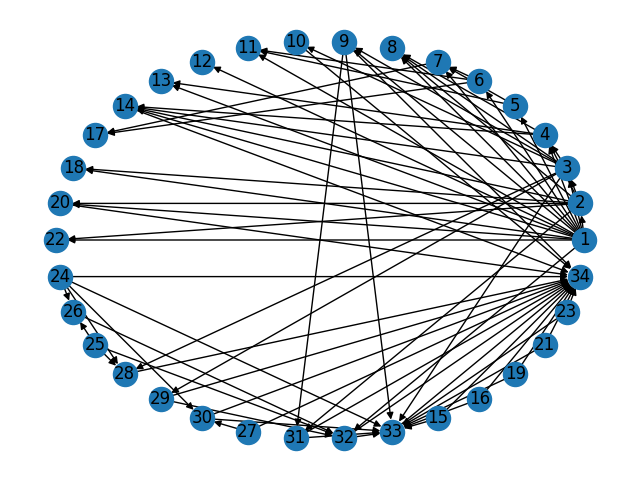
\includegraphics[width=0.4\paperwidth]{imgs/part1.png}
\centering
\end{figure}

\pagebreak

\section{Network collection}

\subsubsection*{Our own network}

We used our own browser history to create network of our most used workflows in the Firefox browser. Nodes in the network are base domain names (eg. \textit{google.com}) and edges represents link clicks.

We have exported browser history from the Firefox SQLite database \textit{places.sqlite} to the \textit{"input/raw\_history\_data.csv"} file with the following query:

\begin{lstlisting}[language=SQL, caption=SQLite query]
SELECT mh.id, from_visit, url
FROM moz_historyvisits mh 
INNER JOIN moz_places mp ON mp.id = mh.place_id
ORDER BY mh.id
\end{lstlisting}

We have constructed the network with the following code:

\begin{lstlisting}[language=Python, caption=src/part2.py]
import csv
import re
import networkx as nx
from statistics import mean 

# read raw data
raw_data = list()
with open("input/raw_history_data.csv") as f:
	raw_data = list(csv.reader(f))

# clean raw data
cleaned_data = dict()
for row in raw_data[1:]:
	visitId = int(row[0])
	fromVisitId = int(row[1])
	url = row[3]

	if(not url.startswith("http")): continue

	match = re.search("^(?:https?:\/\/)?(?:[^@\/\n]+@)?(?:www\.)?([^:\/?\n]+)", url)
	url = url[match.regs[0][0]:match.regs[0][1]]
	domain = url.split("://")[1]
	baseDomain = ".".join(domain.split(".")[-2:])

	cleaned_data[visitId] = {"fromVisitId": fromVisitId, "domain": baseDomain}

# construct weighted edges
edges = dict()
prevNode = {"domain":"/"}
for key in sorted(cleaned_data.keys()):
	node = cleaned_data[key]
	prevNode = cleaned_data.get(node["fromVisitId"], prevNode)
	edge = f"{prevNode['domain']}:{node['domain']}"
	edges[edge] = edges.get(edge, 0) + 1

# build the network
G = nx.DiGraph()
G.add_weighted_edges_from([(*edge.split(":"), weight) for edge,weight in edges.items()])

# print the results
print(f"# nodes: {len(G.nodes)}")
print(f"# edges: {len(G.edges)}")
print(f"avg degree: {mean(map(lambda t: t[1], G.degree()))}")
\end{lstlisting}

This network contains 1123 nodes and 2384 edges with average degree of 4.2.

\subsection*{Synthetic random graph}

We found the equation for the expected number of edges in a network $e = {n\choose 2}*p$, where $n$ denote number of nodes, $p$ the probability of edge creation and $e$ number of edges. Then we have constructed the network with the following code:

\begin{lstlisting}[language=Python, caption=src/part2\_random.py]
import networkx as nx
from statistics import mean 
from scipy.special import binom

# requested number of nodes and edges
N = 1123
E = 2384

# calculate probability p and construct random network
p = E/binom(N, 2)
G = nx.erdos_renyi_graph(N, p, seed=0)

# print the results
print(f"# nodes: {len(G.nodes)}")
print(f"# edges: {len(G.edges)}")
print(f"avg degree: {mean(map(lambda t: t[1], G.degree()))}")
\end{lstlisting}

Randomly constructed network contains 1123 nodes and 2366 edges with average degree of 4.2.

\pagebreak

\section{Network analysis}

We constructed both networks the same way as in the section 2. Then we computed rankings using the PageRank algorithm with the following code:

\begin{lstlisting}[language=Python, caption=src/part3.py]
# ...

# PageRank
rankings = nx.pagerank(G)

# print results
{print(f"{k}: {v:.5f}") for k, v in
    sorted(rankings.items(), key=lambda item: item[1], reverse=True)[:8]}
\end{lstlisting}

And this was the output:

\begin{lstlisting}[caption=Top rankings based on PageRank algorithm]
# Browser history network
duckduckgo.com: 0.06934
google.com: 0.05878
github.com: 0.02372
facebook.com: 0.02005
youtube.com: 0.01093
amazon.de: 0.01035
trello.com: 0.00792
uni-lj.si: 0.00760

# Random generated network
569: 0.00239
454: 0.00229
966: 0.00211
173: 0.00208
178: 0.00206
22: 0.00192
532: 0.00192
438: 0.00187
\end{lstlisting}

We can observe that ranking score drops much faster on the real network compared to the random generated network.

\begin{figure}[h]
\caption{Cropped browser history visualization of the top 200 base domains ranked with PageRank algorithm. Size of the node corresponds to the ranking score.}
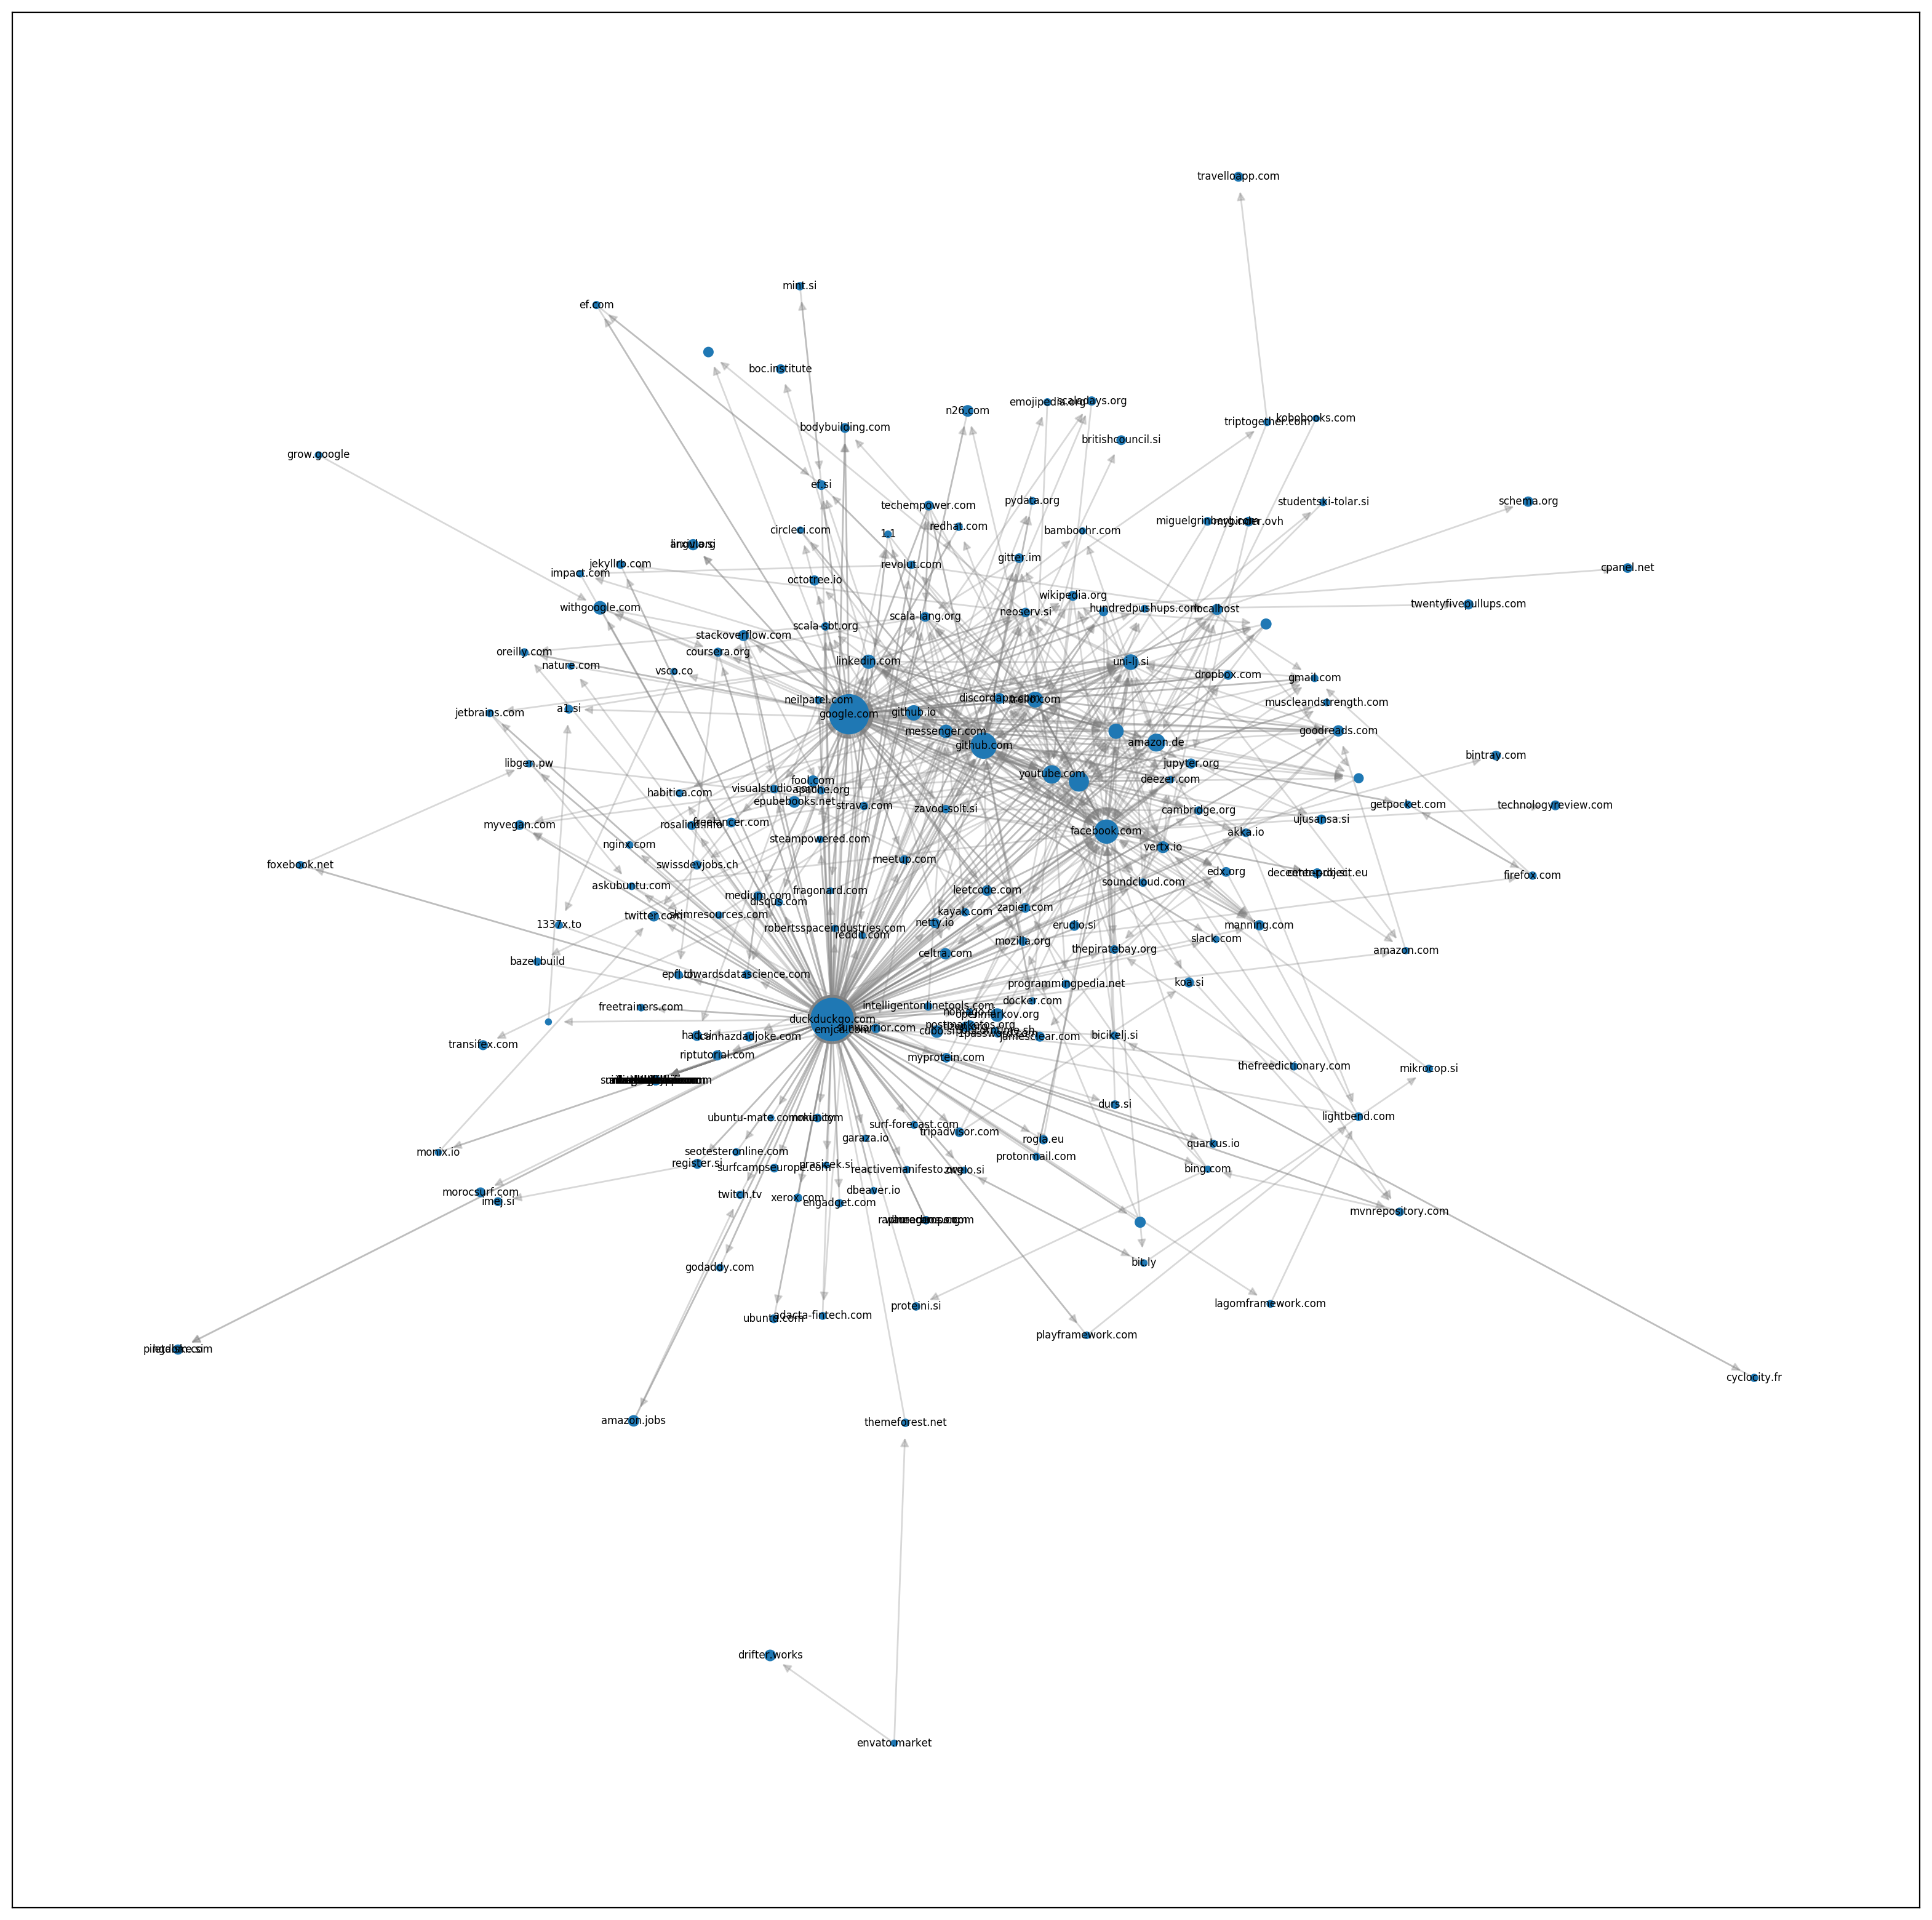
\includegraphics[width=0.75\paperwidth,trim={10cm 10cm 10cm 10cm},clip]{imgs/part3.png}
\centering
\end{figure}

% \bibliographystyle{alpha}
% \bibliography{biblio}

\end{document}
